\chapter{FePd Fit: Version 2}
\label{section:pdfefit2}


This section of the appendix contains the full details of the second version of the Fe-Pd potential.

\FloatBarrier
\section{Potential Files}
\label{section:fepdv2potfiles}

\lstinputlisting[style=sOutputFile,caption={Potential Index File fepd.pot}]{chapters/results_potential_fitting/pot_fepd_fcc_2/fepd.pot}

\lstinputlisting[style=sOutputFile,caption={fe\_pair.pot}]{chapters/results_potential_fitting/pot_fepd_fcc_2/fe_pair.pot}

\lstinputlisting[style=sOutputFile,caption={pd\_pair.pot}]{chapters/results_potential_fitting/pot_fepd_fcc_2/pd_pair.pot}

\lstinputlisting[style=sOutputFile,caption={fepd\_pair.pot}]{chapters/results_potential_fitting/pot_fepd_fcc_2/fepd_pair.pot}


\lstinputlisting[style=sOutputFile,caption={fe\_dens.pot}]{chapters/results_potential_fitting/pot_fepd_fcc_2/fe_dens_slater_4s.pot}

\lstinputlisting[style=sOutputFile,caption={pd\_dens.pot}]{chapters/results_potential_fitting/pot_fepd_fcc_2/pd_dens_slater_4s.pot}


\lstinputlisting[style=sOutputFile,caption={fe\_embe.pot}]{chapters/results_potential_fitting/pot_fepd_fcc_2/fe_embe_ackland.pot}

\lstinputlisting[style=sOutputFile,caption={fe\_embe.pot}]{chapters/results_potential_fitting/pot_fepd_fcc_2/pd_embe_ackland.pot}




\FloatBarrier
\section{Potential Plots}
\label{section:fepdv2potplots}

\FloatBarrier
\begin{figure}[ht] 
  \begin{minipage}[b]{0.5\linewidth}
    \centering
    \includegraphics[width=.9\linewidth]{chapters/results_potential_fitting/pot_fepd_fcc_2/fe_pair.eps} 
    \caption{Fe-Fe Pair Function} 
  \end{minipage}%%
  \begin{minipage}[b]{0.5\linewidth}
    \centering
    \includegraphics[width=.9\linewidth]{chapters/results_potential_fitting/pot_fepd_fcc_2/fe_pair_zoom.eps} 
    \caption{Fe-Fe Pair Function (Zoomed In)} 
  \end{minipage} 
  \begin{minipage}[b]{0.5\linewidth}
    \centering
    \includegraphics[width=.9\linewidth]{chapters/results_potential_fitting/pot_fepd_fcc_2/fe_dens_slater_4s.eps} 
    \caption{Fe Density Function} 
  \end{minipage}%% 
  \begin{minipage}[b]{0.5\linewidth}
    \centering
    \includegraphics[width=.9\linewidth]{chapters/results_potential_fitting/pot_fepd_fcc_2/fe_embe_ackland.eps} 
    \caption{Fe Embedding Function} 
  \end{minipage} 
  \label{fig:ironFCCPotentialPlots} 
\end{figure}
\FloatBarrier


\begin{figure}[ht] 
  \begin{minipage}[b]{0.4\linewidth}
    \centering
    \includegraphics[width=.9\linewidth]{chapters/results_potential_fitting/pot_fepd_fcc_2/pd_pair.eps} 
    \caption{Pd-Pd Pair Function}  
  \end{minipage}%%
  \begin{minipage}[b]{0.4\linewidth}
    \centering
    \includegraphics[width=.9\linewidth]{chapters/results_potential_fitting/pot_fepd_fcc_2/pd_pair_zoom.eps} 
    \caption{Pd-Pd Pair Function (Zoomed In)} 
  \end{minipage} 
  \begin{minipage}[b]{0.4\linewidth}
    \centering
    \includegraphics[width=.9\linewidth]{chapters/results_potential_fitting/pot_fepd_fcc_2/pd_dens_slater_4s.eps} 
    \caption{Pd Density Function} 
  \end{minipage}%% 
  \begin{minipage}[b]{0.4\linewidth}
    \centering
    \includegraphics[width=.9\linewidth]{chapters/results_potential_fitting/pot_fepd_fcc_2/pd_embe_ackland.eps} 
    \caption{Pd Embedding Function} 
  \end{minipage} 
  \label{fig:ironPotentialPlots} 
\end{figure}

\begin{figure}[ht] 
  \begin{minipage}[b]{0.4\linewidth}
    \centering
    \includegraphics[width=.9\linewidth]{chapters/results_potential_fitting/pot_fepd_fcc_2/pd_pair.eps} 
    \caption{Fe-Pd Pair Function}  
  \end{minipage}%%
  \begin{minipage}[b]{0.4\linewidth}
    \centering
    \includegraphics[width=.9\linewidth]{chapters/results_potential_fitting/pot_fepd_fcc_2/fepd_pair.eps} 
    \caption{Fe-Pd Pair Function (Zoomed In)}  
  \end{minipage}%%
\end{figure}


\FloatBarrier
\section{Equation of State and Elastic Constant (Distortion) Plots}
\label{section:fepdv2eosec}


\begin{figure}[ht] 
  \begin{minipage}[b]{0.4\linewidth}
    \centering
    \includegraphics[width=.9\linewidth]{chapters/results_potential_fitting/pot_fepd_fcc_2/fe_eos_1.eps} 
    \caption{Iron equation of state}  
  \end{minipage}%%
  \begin{minipage}[b]{0.4\linewidth}
    \centering
    \includegraphics[width=.9\linewidth]{chapters/results_potential_fitting/pot_fepd_fcc_2/fe_ec_1.eps} 
    \caption{Iron elastic constants}  
  \end{minipage}%%
\end{figure}


\begin{figure}[ht] 
  \begin{minipage}[b]{0.4\linewidth}
    \centering
    \includegraphics[width=.9\linewidth]{chapters/results_potential_fitting/pot_fepd_fcc_2/pd_eos_0.eps} 
    \caption{Palladium equation of state}  
  \end{minipage}%%
  \begin{minipage}[b]{0.4\linewidth}
    \centering
    \includegraphics[width=.9\linewidth]{chapters/results_potential_fitting/pot_fepd_fcc_2/pd_ec_0.eps} 
    \caption{Palladium elastic constants}  
  \end{minipage}%%
\end{figure}


\FloatBarrier
\section{Cohesive Energy Plots}
\label{section:fepdv2coh}


\begin{figure}[ht] 
  \begin{minipage}[b]{0.4\linewidth}
    \centering
    \includegraphics[width=.9\linewidth]{chapters/results_potential_fitting/pot_fepd_fcc_2/fe_cohesive_energy.eps} 
    \caption{Iron cohesive energy}  
    \label{fig:fev2cohesive}
  \end{minipage}%%
  \begin{minipage}[b]{0.4\linewidth}
    \centering
    \includegraphics[width=.9\linewidth]{chapters/results_potential_fitting/pot_fepd_fcc_2/fe_cohesive_energy_zoom.eps} 
    \caption{Iron cohesive energy (zoomed in)}  
    \label{fig:fev2cohesivezoom}
  \end{minipage}%%
\end{figure}

\begin{figure}[ht] 
  \begin{minipage}[b]{0.4\linewidth}
    \centering
    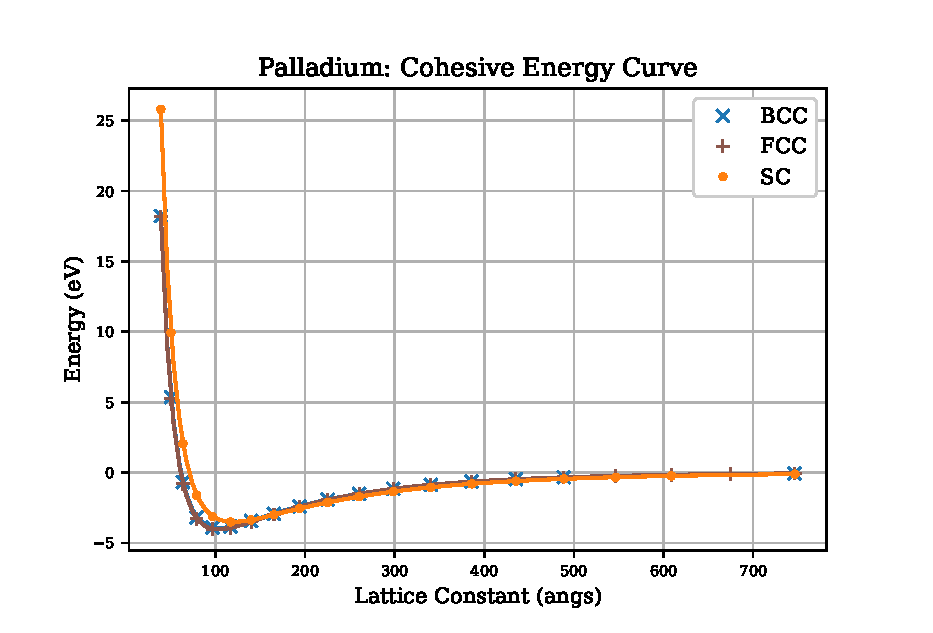
\includegraphics[width=.9\linewidth]{chapters/results_potential_fitting/pot_fepd_fcc_2/pd_cohesive_energy.eps} 
    \caption{Palladium cohesive energy}  
    \label{fig:pdv2cohesive}
  \end{minipage}%%
  \begin{minipage}[b]{0.4\linewidth}
    \centering
    \includegraphics[width=.9\linewidth]{chapters/results_potential_fitting/pot_fepd_fcc_2/pd_cohesive_energy_zoom.eps} 
    \caption{Palladium cohesive energy (zoomed in)}
    \label{fig:pdv2cohesivezoom}  
  \end{minipage}%%
\end{figure}


\FloatBarrier
\section{Surface Energy Plots}
\label{section:fepdv2se}

\begin{figure}[ht] 
  \begin{minipage}[b]{0.4\linewidth}
    \centering
    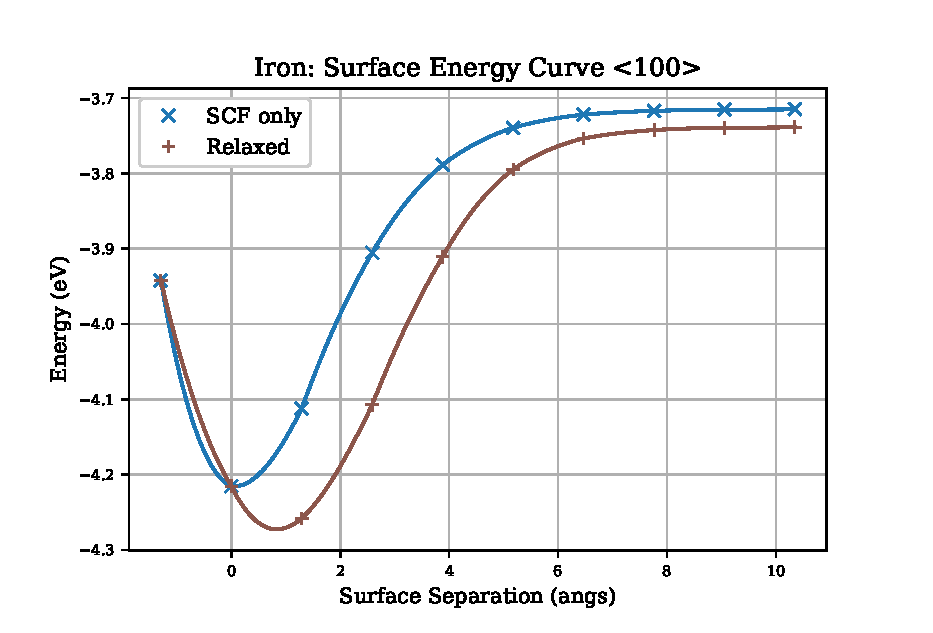
\includegraphics[width=.9\linewidth]{chapters/results_potential_fitting/pot_fepd_fcc_2/fe_surface_energy.eps} 
    \caption{Iron surface energy}  
    \label{fig:fev2surface}
  \end{minipage}%%
  \begin{minipage}[b]{0.4\linewidth}
    \centering
    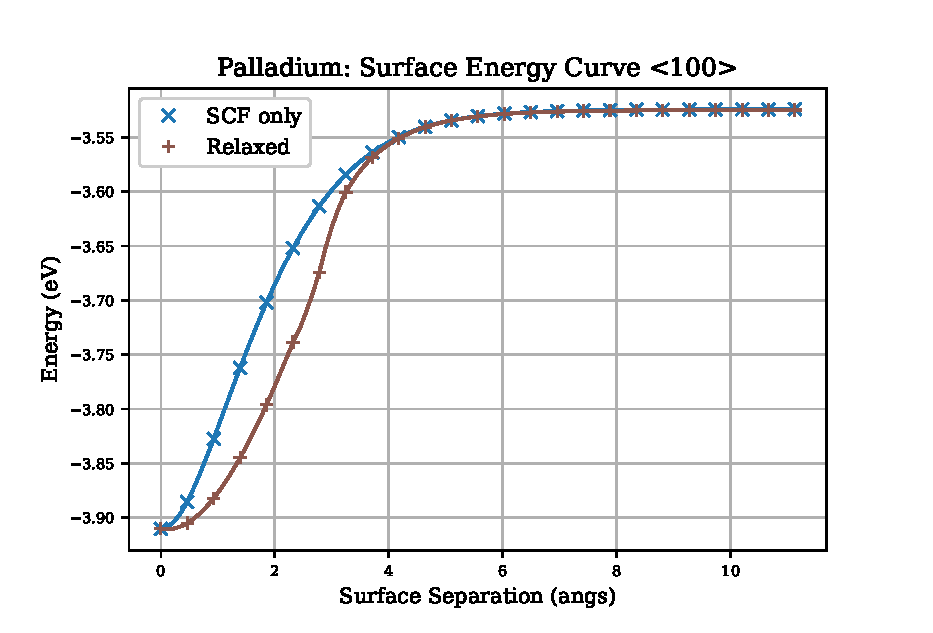
\includegraphics[width=.9\linewidth]{chapters/results_potential_fitting/pot_fepd_fcc_2/pd_surface_energy.eps} 
    \caption{Palladium surface energy}  
    \label{fig:pdv2surface}
  \end{minipage}%%
\end{figure}



\FloatBarrier
\section{Fe-Pd V2 Potential Properties}

\begin{table}[ht]
\renewcommand{\arraystretch}{1.2}
\begin{tabular}{lcc}
\hline\hline
Parameter & Experimental/DFT & This Potential\\
\hline\hline
$a_0$ & 3.42   &  3.40  \\
$e_0$ & -4.27  & -4.29  \\
$B_0$ & 222.0  &  229.1  \\
$C_{11}$ & 365.6  &  365.9 \\
$C_{22}$ & 298.7  &  298.6 \\
$C_{33}$ & 364.0  &  365.9 \\
$C_{44}$ & 186.3  &  187.6  \\
$C_{55}$ & 266.8  &  258.4 \\
$C_{66}$ & 186.3  &  187.6 \\
$C_{12}$ & 141.6  &  141.1 \\
$C_{13}$ & 233.8  &  238.1 \\
$C_{23}$ & 130.4  &  124.8 \\
\hline\hline
\end{tabular}
\label{tab:ironpotpropertiesv2}
\caption{Iron potential properties (experimental vs this work v2)}
\end{table}

\begin{table}[ht]
\renewcommand{\arraystretch}{1.2}
\begin{tabular}{lcc}
\hline\hline
Parameter & Experimental/DFT & This Potential\\
\hline\hline
$a_0$ & 3.89 & 3.87  \\
$e_0$ & -3.91  & -3.91  \\
$B_0$ & 180.0  & 171.3  \\
$C_{11}$ & 234.0  & 232.9  \\
$C_{12}$ & 176.0  & 176.7  \\
$C_{44}$ & 71.2  & 68.8  \\
\hline\hline
\end{tabular}
\label{tab:palladiumpotpropertiesv2}
\caption{Palladium potential properties (experimental vs this work v2)}
\end{table}















